\documentclass{../exhibit}

\title{Plundered Treasure}

%% Font
\usepackage{imfellEnglish}
\usepackage[T1]{fontenc}
\raggedright

\usepackage[LGRgreek]{mathastext}


%% so title is accessable
\makeatletter
\let\thetitle\@title
\let\theabstract\@abstract
\makeatother


\usepackage{background}
\backgroundsetup{
scale=1,
color=white,
opacity=0.2,
angle=0,
contents={%
  \hspace{0 in}\raisebox{0 in}{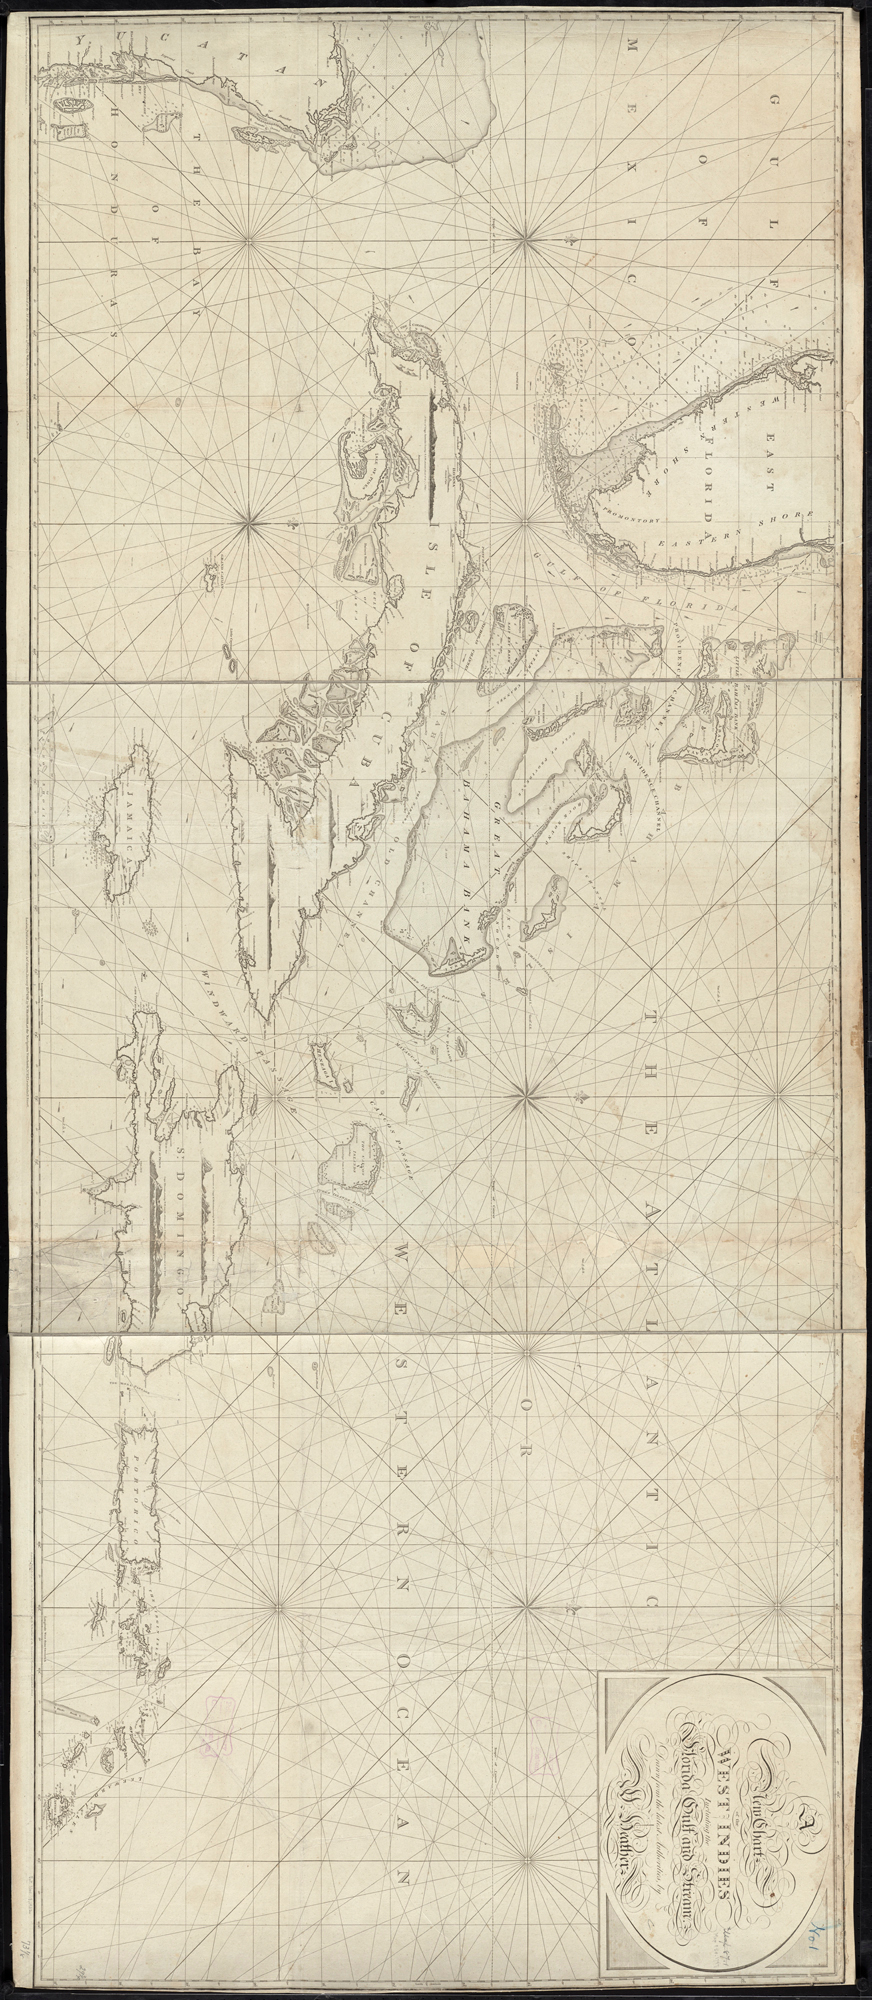
\includegraphics[scale=.5]{mapBackground.jpg}}
  %%https://commons.wikimedia.org/wiki/File:1683_Mortier_Map_of_North_America,_the_West_Indies,_and_the_Atlantic_Ocean_-_Geographicus_-_Atlantique-mortier-1693.jpg
  }%
}


\def\imagetop#1{\vtop{\null\hbox{#1}}}

%% For the context
%% https://tex.stackexchange.com/questions/86150/torn-page-effect/86151#86151
\usepackage{tikz}
\usetikzlibrary{decorations.pathmorphing}
\definecolor{paper}{RGB}{239,227,157}


%% QR code
\usepackage{qrcode}



%% For bold-ish title
\usepackage{shadowtext}



\renewcommand{\maketitle}{ %
  \shadowoffset{.5pt} %% See: https://tex.stackexchange.com/questions/159463/fancy-styled-borders-in-latex
  \shadowcolor{black!50!white}
  \begin{center}
    \resizebox{\textwidth}{!}{\shadowtext{\scshape\thetitle}}
  \end{center}
  
\vspace{1cm}
  
\begin{tabular*}{\textwidth}{c @{\extracolsep{\fill}} c}  
  \imagetop{
\begin{tikzpicture}
        \node[preaction={fill=white,opacity=0},inner sep=.5cm] 
             {
               \begin{minipage}{.45\textwidth}\Huge\directions\end{minipage}
             };
  \end{tikzpicture}}
  &
  \imagetop{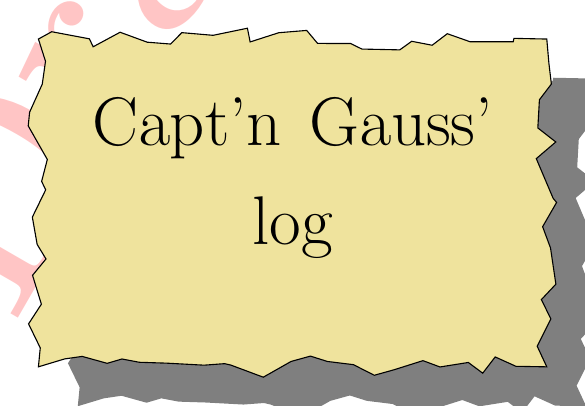
\begin{tikzpicture}[pencildraw/.style={ %%% https://tex.stackexchange.com/questions/86150/torn-page-effect/86151#86151
            decorate,
            decoration={random steps,segment length=8pt,amplitude=4pt}
          } %
        ]
        \node[preaction={fill=black,opacity=.5,transform canvas={xshift=.5cm,yshift=-.5cm}},pencildraw,draw,fill=paper,text width=.45\textwidth,inner sep=.5cm]
             {
               \vspace{-.7cm}
               \begin{center}\HUGE Capt'n \ \ Gauss' \ \  log \end{center}\vspace{.6cm} {\Huge\textit\context}
             };
  \end{tikzpicture}}
  
\end{tabular*}

\vfill



\begin{tikzpicture}
  \node[preaction={fill=white,opacity=0},inner sep=.5cm] 
             {
               \begin{minipage}{\textwidth}\Huge\example\end{minipage}
             };
  \end{tikzpicture}





\vfill


\includegraphics[width=2in]{bammLogo.png}
\hfill

\includegraphics[width=3in]{logoPirate.png}
\hfill
\raisebox{2cm}{\begin{tabular}{c}
\huge How's this math? \\
\qrcode[height=1.5in]{\mathConnections}
\end{tabular}}

}


\begin{document}

\begin{context} I need your help\dots


Move all the treasure disks from


\quad ``Treasure Island''

\quad \quad \quad\quad to the


\quad \quad \quad \quad \quad ``Pirate Ship''




using the ``Port'' as a
temporary holding area.


Use the ``Port'' wisely!
\end{context}

\begin{directions}
\begin{itemize}
\item The left most tower is the ``Island.''
\item The middle post is the ``Port.''
\item The final post is the ``Ship.''
\end{itemize}

Place treasure disks on the ``Island'' tower in order with the largest
at the bottom and the smallest at the top.
\begin{itemize}
\item Move one treasure disk at a time, move it to any where you want
  BUT
\item Never place a larger treasure disk on top of a smaller one.
\end{itemize}
You WIN when all the treasure is on the SHIP!
\end{directions}


\begin{example}
  The initial configuration might look like this:
  \begin{center}
    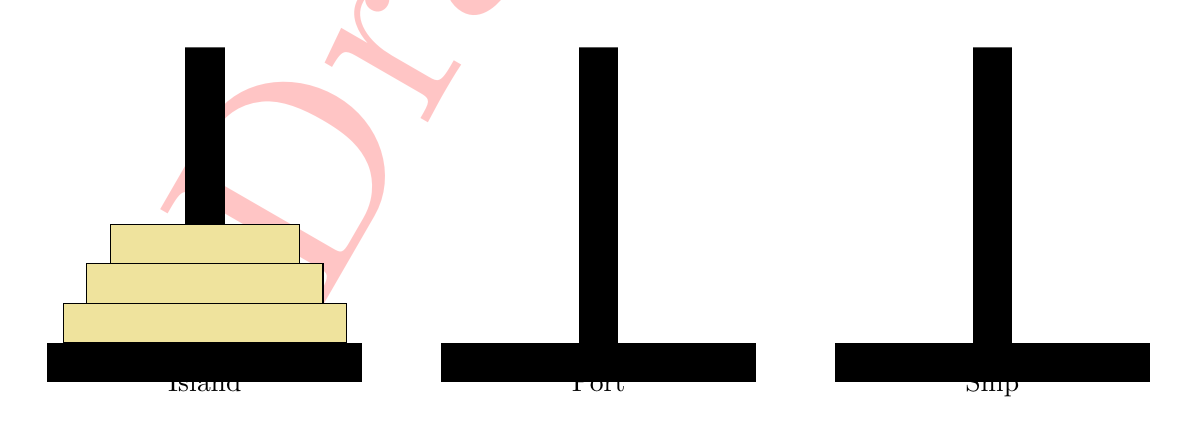
\begin{tikzpicture}
    % Draw the three towers
    \draw[line width = .5cm] (0,0) -- (2,0) -- (2,4) -- (2,0) -- (4,0);
    \draw[line width = .5cm] (5,0) -- (7,0) -- (7,4) -- (7,0) -- (9,0);
    \draw[line width = .5cm] (10,0) -- (12,0) -- (12,4) -- (12,0) -- (14,0);

    \filldraw[fill=paper] (.2,.25) rectangle (3.8,.75);
    \filldraw[fill=paper] (.5,.75) rectangle (3.5,1.25);
    \filldraw[fill=paper] (.8,1.25) rectangle (3.2,1.75);
    
    % Draw labels
    \node[below] at (2,0) {Island};
    \node[below] at (7,0) {Port};
    \node[below] at (12,0) {Ship};
\end{tikzpicture}
%% \begin{tikzpicture}
%%     % Draw the three towers
%%     \draw (0,0) -- (0,3) -- (1,3) -- (1,0) -- cycle;
%%     \draw (3,0) -- (3,3) -- (4,3) -- (4,0) -- cycle;
%%     \draw (6,0) -- (6,3) -- (7,3) -- (7,0) -- cycle;

%%     % Draw the disks
%%     \filldraw[fill=white] (0.5,2.1) circle (0.2);
%%     \filldraw[fill=white] (0.5,1.4) circle (0.3);
%%     \filldraw[fill=white] (0.5,0.5) circle (0.4);

%%     % Draw labels
%%     \node at (0.5,3.5) {Island};
%%     \node at (3.5,3.5) {Port};
%%     \node at (6.5,3.5) {Ship};
%% \end{tikzpicture}
\end{center}
\end{example}


\begin{mathConnections}
  https://bartsnapp.github.io/Math-Outreach-Exhibits/towersOfHanoi/
\end{mathConnections}

\end{document}
